\documentclass[12pt,twoside]{article}
\usepackage{amsmath, amssymb}
\usepackage{amsmath}
\usepackage{fancyhdr,parskip}
\usepackage[active]{srcltx}
\usepackage{amssymb}
\usepackage{amscd}
\usepackage{makeidx}
\usepackage{amsthm}
\usepackage{algorithm}
\usepackage{algpseudocode}
\usepackage{fancyhdr}
\usepackage{graphics}
\usepackage{amsmath, amssymb}
\usepackage{amsmath}
\usepackage[active]{srcltx}
\usepackage{amssymb}
\usepackage{amscd}
\usepackage{makeidx}
\usepackage[dvips]{graphicx}
\usepackage{longtable}
\usepackage{tabularx}
\usepackage[table,xcdraw]{xcolor}
\usepackage{color}
\usepackage[hidelinks]{hyperref}
\usepackage[backend=biber,style=apa]{biblatex}
\usepackage{longtable}
\usepackage{tabularx}
\usepackage[table,xcdraw]{xcolor}
\usepackage{color}
\usepackage[hidelinks]{hyperref}
\usepackage{multirow}
\usepackage{algorithm}
\usepackage{algpseudocode}
\usepackage{fancyhdr,graphicx,amsmath,amssymb}
\renewcommand{\algorithmicrequire}{\textbf{Input:}}
\renewcommand{\algorithmicensure}{\textbf{Output:}}
\renewcommand{\tablename}{Tabla}
\renewcommand{\figurename}{Figura}
\renewcommand{\baselinestretch}{1}
\setcounter{page}{1}
\setlength{\textheight}{21.6cm}
\setlength{\textwidth}{14cm}
\setlength{\oddsidemargin}{1cm}
\setlength{\evensidemargin}{1cm}
\pagestyle{myheadings}
\thispagestyle{empty}
\markboth{\small{Pr\'actica 6. Luis Francisco Renteria Cedillo, Denzel Omar Vazquez Perez.}}{\small{.}}
\date{}
\begin{document}
\begin{figure}[h]
    \vspace{-3cm} \hspace{-2cm} \setlength{\unitlength}{1mm}
    \begin{picture}(15,25)(-10,0)
    
\includegraphics[width=16.5cm,height=2.8cm]{imagenes/titulo.png}
    \end{picture}
    \end{figure}
    \vspace{0cm}
    \centerline{\bf An\'alisis de Algoritmos, Sem: 2022-2, 3CV11, Pr\'actica 6, 07 de junio de 2022}
    \centerline{}
    \begin{center}
    \Large{\textsc{Pr\'actica 6: Programaci\'on Din\'amica}}
    \end{center}
    \centerline{}
    \centerline{\bf {Luis Francisco Renteria Cedillo, Denzel Omar Vazquez Perez.}}
    \centerline{}
    \centerline{$lrenteriac1400@alumno.ipn.mx, dvazquezp1600@alumno.ipn.mx$}
    \newtheorem{Theorem}{\quad Theorem}[section]
    \newtheorem{Definition}[Theorem]{\quad Definition}
    \newtheorem{Corollary}[Theorem]{\quad Corollary}
    \newtheorem{Lemma}[Theorem]{\quad Lemma}
    \newtheorem{Example}[Theorem]{\quad Example}
    \bigskip

\textbf{Resumen:} En el presente documento se muestra la aplicación del algoritmo "Subsecucia Común mas Larga" con el objetivo de comparar dos archivos de código fuente en C y obtener un porcentaje de puntuación de similitud.\\

{\bf Palabras Clave:}Antiplagio, Programación Dinámica, Expresiones Regulares, Python

\section{Introducci\'on}
    Se entiende como plagio el copiar, imitar y/o atribuirse una obra que no es de nuestra autoría, violando uno de los derechos morales el cual es el derecho patrimonial de la obra. En términos académicos, el hacer plagio es considerado como una falta ética y en la mayoría de los casos es fuertemente sancionado, ya que conlleva la intención de engañar a una comunidad y robar una obra ajena para obtener un beneficio o ventaja.  Sin embargo, existe el derecho de citar al autor a pequeñas partes de una obra, siempre y cuando no se considere una reproducción sustancial de la misma.\\

    Una herramienta popular en universidades e institutos es el software Turnitin, el cual es un servicio de prevención de plagio, utilizado en mas de 140 países y alrededor de 15,000 instituciones. Dicha herramienta fue creada a finales de los años 90 por estudiantes de la Universidad de California en Berkley. Su objetivo principal fue el facilitar la corrección por pares y en 2002 fue constituido Turnitin como se conoce hoy en día.\\

    El funcionamiento básico de Turnitin es el siguiente: el usuario manda un archivo de texto al servicio de Turnitin, el cual se procesa y se calcula un porcentaje de similitud respecto a la base de datos interna de Turnitin. De esta manera, los profesores pueden revisar los trabajos de los alumnos de manera automatizada y decidir si una obra es plagiada o no.
    
\section{Conceptos B\'asicos}
    \subsection{Expresiones Regulares}
        En teoría de la computación, una expresión regular se utiliza para realizar una búsqueda en una cadena de texto conforme a un patrón, empleando una combinación de caracteres. Dicho de otra forma, las expresiones regulares brindan una manera muy flexible para reconocer cadenas de texto.
        Existen tres operadores que se utilizan en la construcción de las expresiones regulares: unión, concatenación y cerradura de Kleene.
        
    \subsection{Programaci\'on din\'amica}
        La programación dinámica es un enfoque algorítmico para buscar la solución de un problema de optimización dividiéndolo en varios subproblemas más simples, observando que el problema global depende de la solución óptima de sus subproblemas. Por lo tanto, la característica más esencial de programación dinámica es la estructura adecuada de los problemas de optimización en múltiples niveles, que se resuelven secuencialmente a un nivel a la vez.\\ Mediante el uso de técnicas ordinarias de problemas de optimización, se resuelve cada nivel y su solución ayuda a definir las características del problema del siguiente nivel en la secuencia. Comúnmente, los niveles representan diferentes periodos de tiempo en la perspectiva del problema general.
        \\
    \subsection{Algoritmo de la Subsecucia Común mas Larga}
        Algoritmo es usado para encontrar la subsecuencia com\'n m\'as larga entre dos cadenas de caracteres. Dicha subsecuencia no necesariamente tiene que ser contigua en ambas cadenas.
\newpage
\section{Experimentaci\'on y Resultados}
    \subsection{An\'alisis a Priori}
    Dada la implementaci\'on del algoritmo de la subsecucia com\'un mas larga en el lenguaje de programaci\'on Python se muestra en la Figura 1, la codificaci\'on de este.\\
    Entonces sea cada bloque de secuencias del c\'odigo, se determina el orden de complejidad del para el peor caso de este por medio por medio del an\'alisis de segmentos de c\'odigo concluyendo que el algoritmo tiene orden de complejidad $T(n)\in\Theta(mn)$.
    \begin{figure}[H]
        \centering
        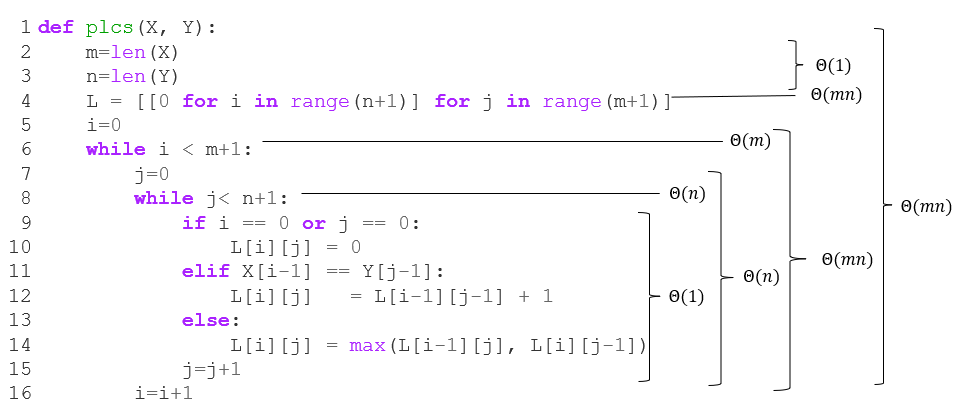
\includegraphics[width=14cm]{imagenes/lcs.png}
        \caption{Análisis por bloques de c\'odigo del algoritmo}
    \end{figure}
    \subsection{Resultados}
    Con ayuda del algoritmo de la subsecucia com\'un mas larga, se pone en pr\'actica en un programa que comparar dos archivos de c\'odigo fuente en lenguaje C con el prop\'osito de detectar el porcentaje de coincidencias que puedan tener.
    
    A continiaci\'on se muestran los resultados a partir de archivos en los que solo se hizo cambios de nombres a variables asi como c\'odigos totalmente distintos.
    
    Para el primer caso se escogi\'o el archivo {\it NQueens.c}, con el objetivo de comparar el mismo archivo y obtener el 100\% de las coincidencias puesto que se analiza el mismo c\'odigo fuente, as\'i en la Figura 2 se aprecia que se logro obtener lo esperado.
    \begin{figure}[H]
        \centering
        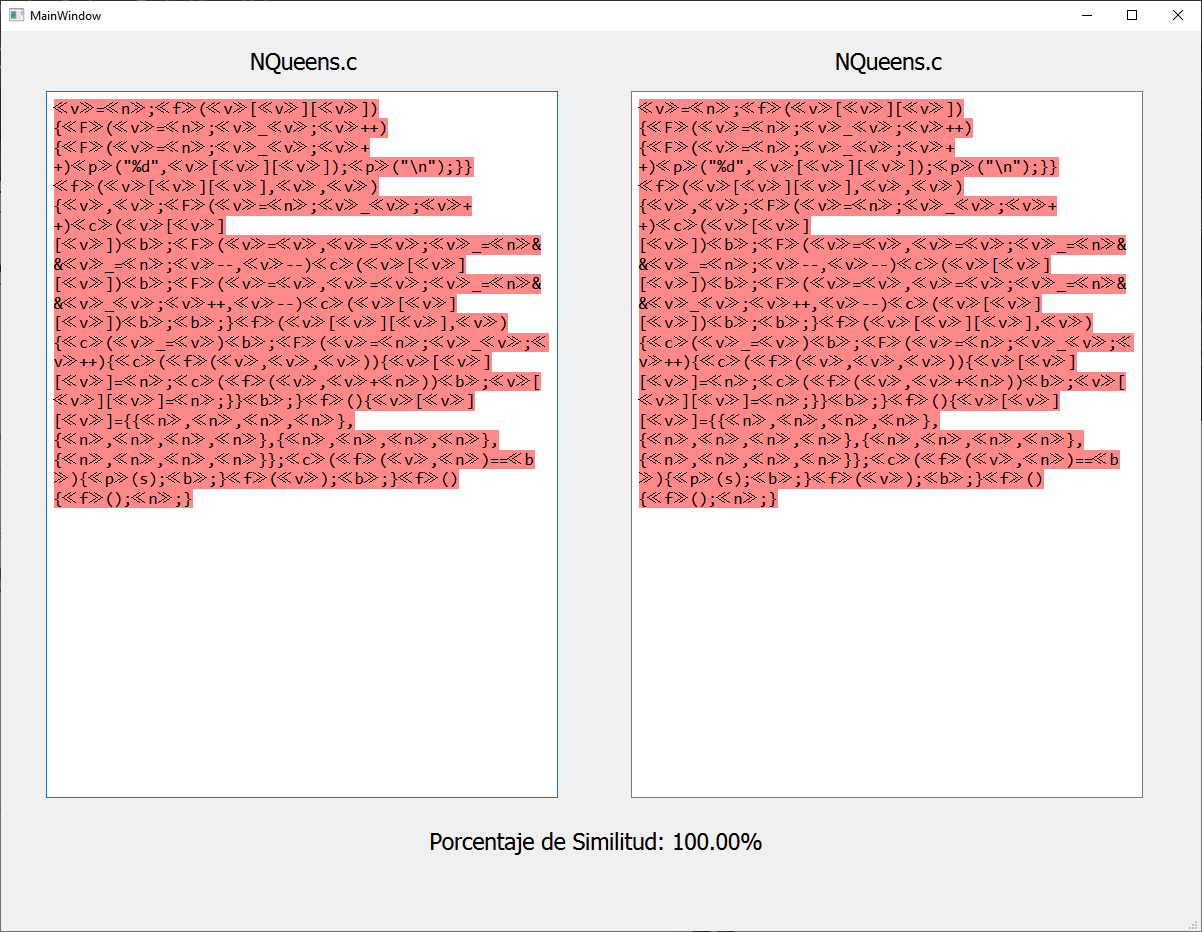
\includegraphics[width=9cm]{imagenes/i1.png}
        \caption{Prueba con el mismo archivo de c\'odigo fuente}
    \end{figure}
    El siguiente caso se selecciono y modifico haciendo el cambio al nombre de las variables de {\it NQueens.c}, este archivo se nombro {\it NQueensPlagio.c}, as\'i en la Figura 3 el programa implementado detecta que el programa sigue siendo el mismo aun cambiando el nombre de la variables del c\'odigo fuente, por tanto el porcentaje de coincidencia es del 100\%.
    \begin{figure}[H]
        \centering
        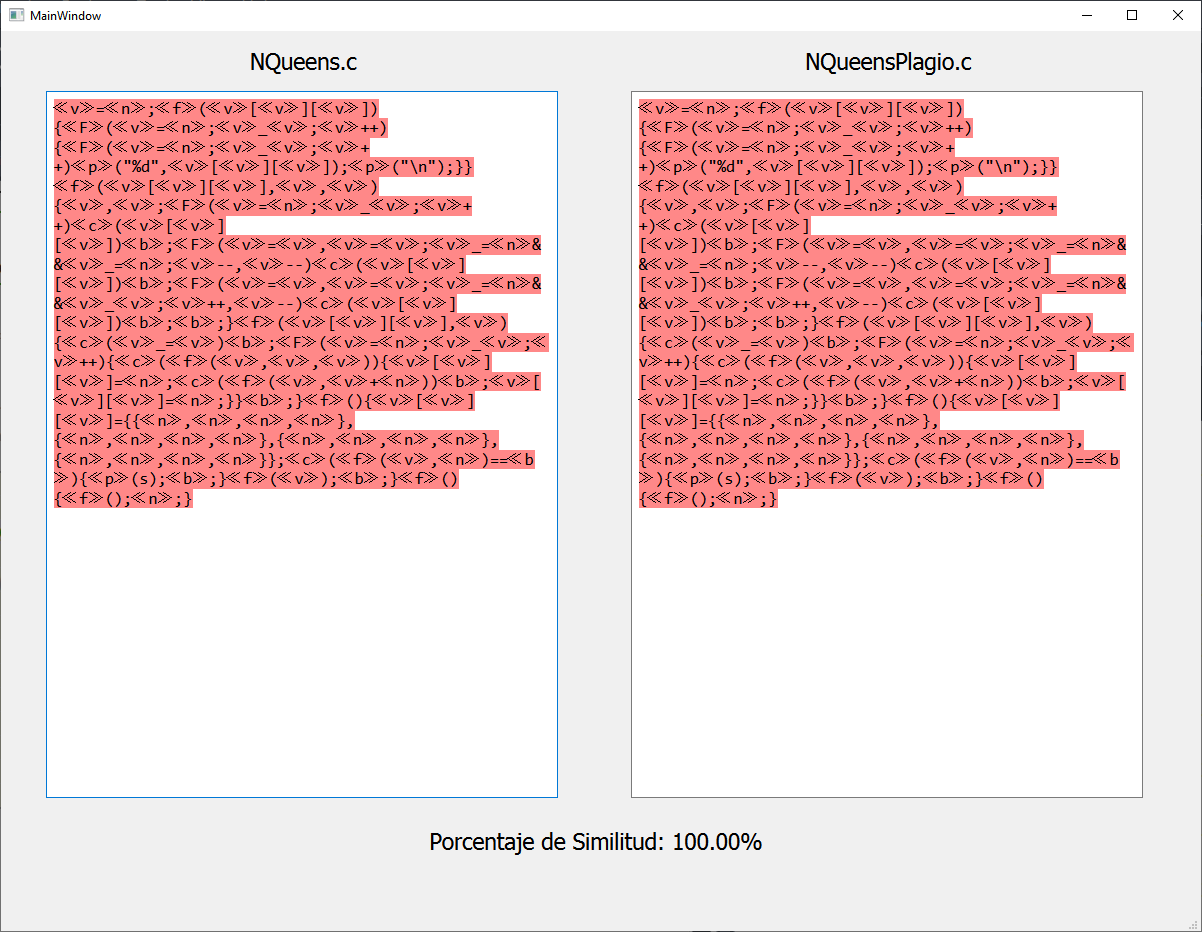
\includegraphics[width=9cm]{imagenes/i2.png}
        \caption{Prueba con el cambio del nombre de las variables}
    \end{figure}
    Para el tercer y ultimo caso, se hace uso de dos archivos de c\'odigo fuente totalmente distintos, para verificar que el porcentaje de coincidencia sea inferior existiendo coincidencias m\'inimas entre estos. Asi en la Figura 4 se muestra que los archivos {\it heap\_sort.c} y {\it quick.c} tienen un porcentaje de coincidencia del 18.38\%.
    \begin{figure}[H]
        \centering
        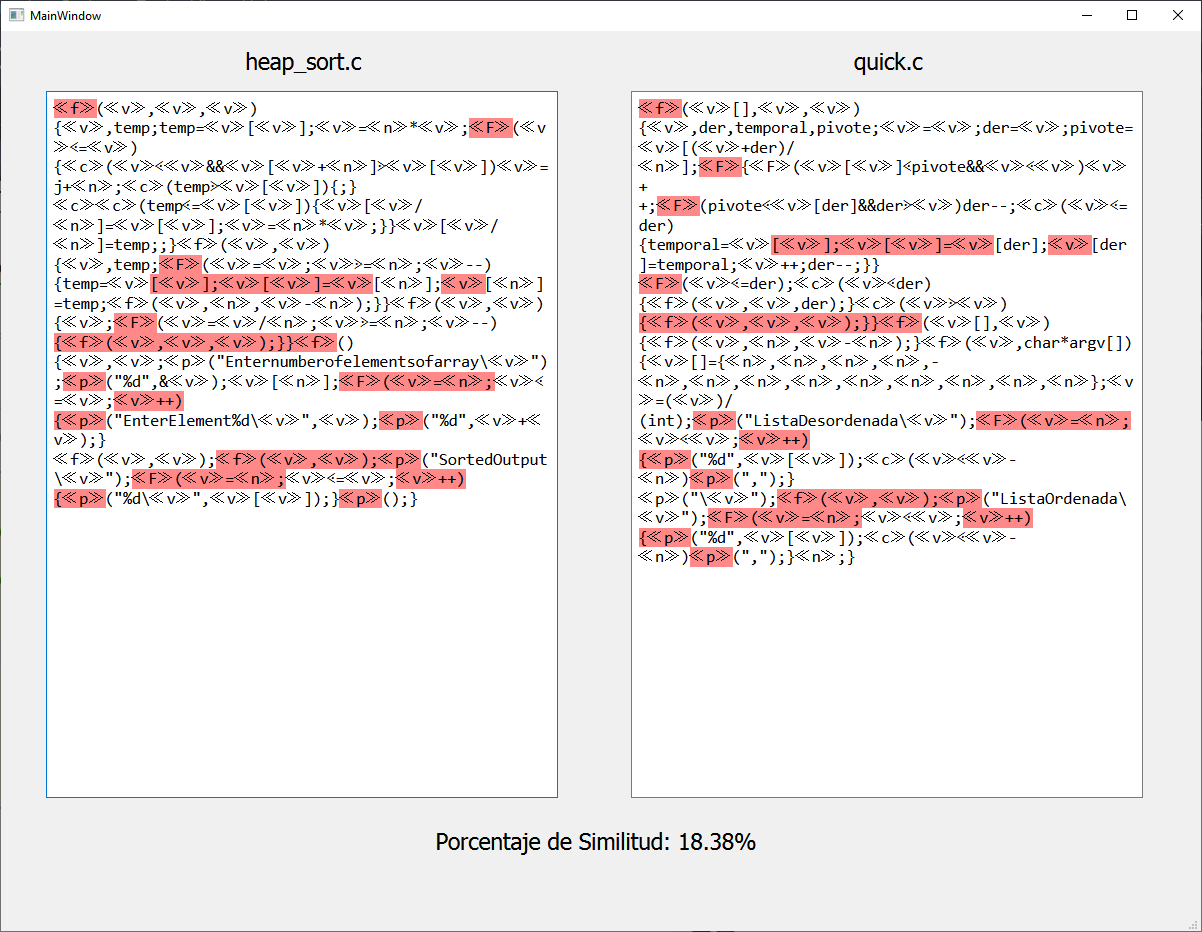
\includegraphics[width=9cm]{imagenes/i3.png}
        \caption{Primer prueba con distintos archivos}
    \end{figure}
    Para Figura 5 se muestra el segundo ejemplo donde los archivos {\it merge.c} y {\it quick.c} son diferentes y presentan un porcentaje de coincidencia del 14.56\%.
    \begin{figure}[H]
        \centering
        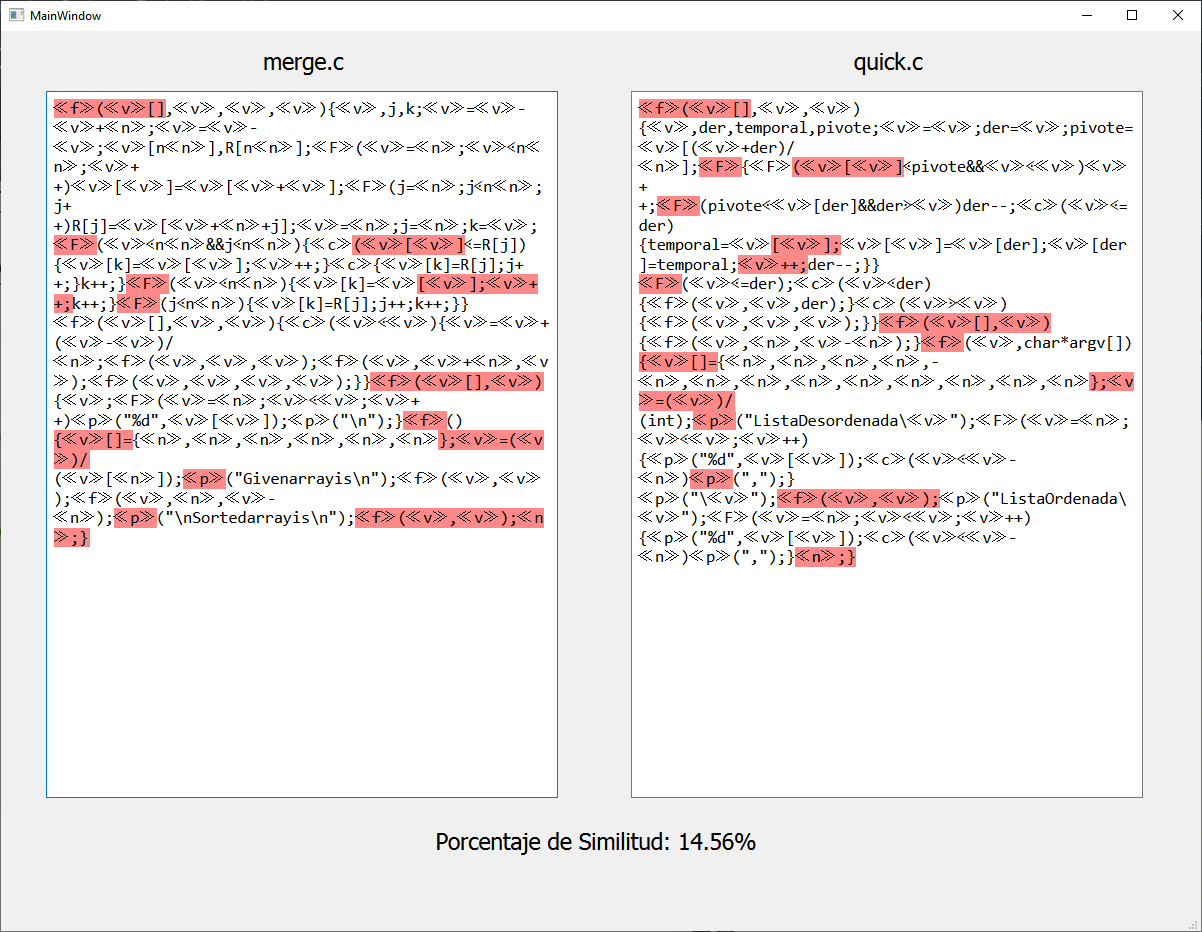
\includegraphics[width=9cm]{imagenes/i4.png}
        \caption{Segunda prueba con distintos archivos}
    \end{figure}
    Finalmente en la Figura 6 se muestra el tercer ejemplo que hace uso de un archivo extra\'ido de internet  y uno en el que se trabajo , {\it dijkstra.c} y {\it dijkstra2.c} respectivamente, teniendo un porcentaje de coincidencia del 22.78\%.
    \begin{figure}[H]
        \centering
        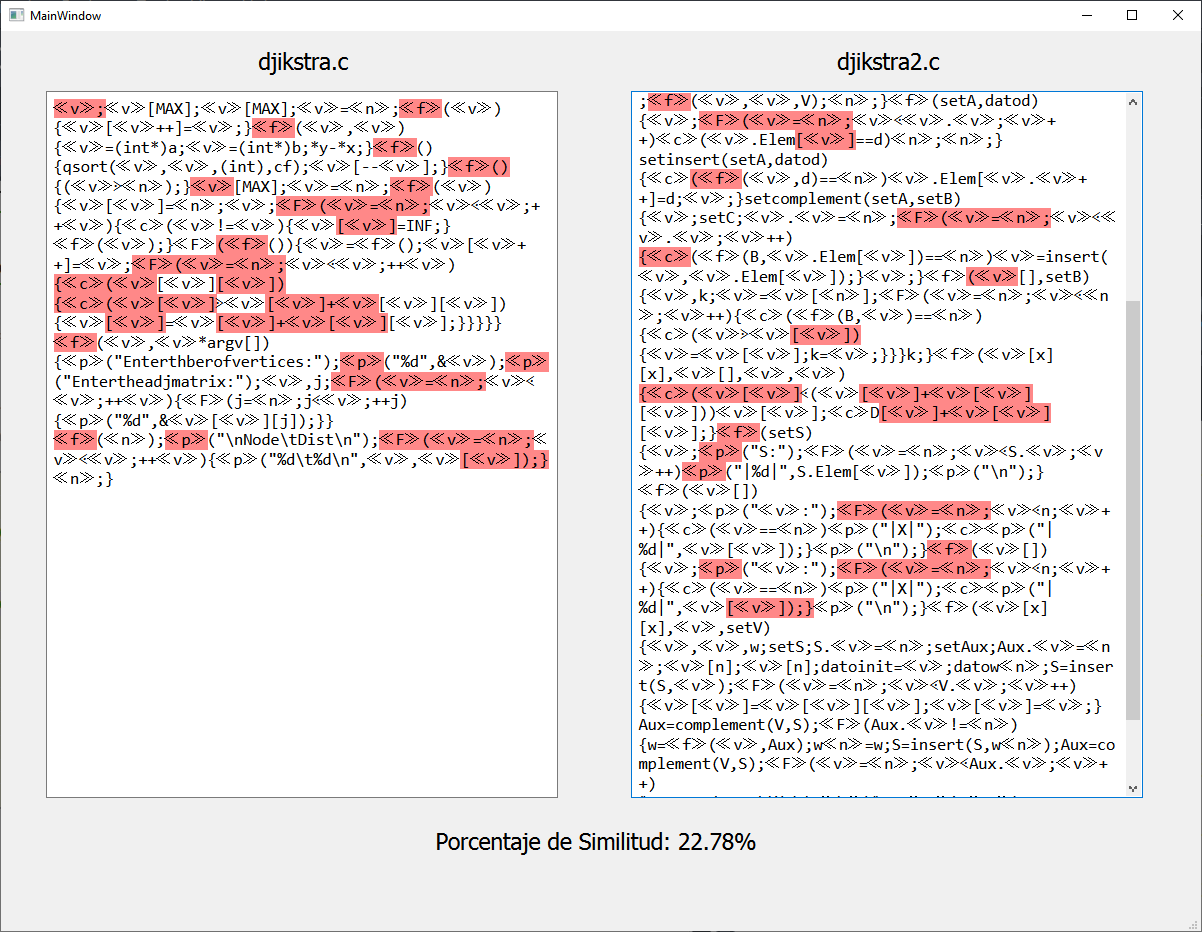
\includegraphics[width=9cm]{imagenes/i5.png}
        \caption{Tercer prueba con distintos archivos}
    \end{figure}
    El programa resulta eficaz, puesto al tokenizar los archivos con los que se trabaja es posible cambiar las palabras reservadas de lenguaje C usando literales que denotan el tipo de sentencia que se esta manejando en el instante gracias a expresiones regulares, as\'i al finalizar cambio antes comentado se implementa el algoritmo de la subsecuencia com\'un mas larga, mostrando las coincidencias encontradas marcadas con color rojo en el proceso. As\'i se determina que para detectar el plagio es necesario encontrar la frase mas larga compartida, dado que las frases son cadenas de caracteres consecutivos y aquí se necesita la subsecuencia común más larga entre los c\'odigos fuente.
\newpage
\section{Conclusiones}

    \textbf{\large Luis Francisco Renteria Cedillo}
        \begin{figure}[H]
            \centering
            
\includegraphics[angle=0, scale=0.5]{imagenes/foto1.png}
        \end{figure}
    Cuando implementamos la búsqueda de la subsecuencia común más larga, en su primer versión, nos percatamos que el porcentaje era muy alto aún cuando los códigos eran totalmente distintos, esto se debe a que en nuestro código, en su versión inicial, identificaba cada carácter como un elemento, por tal motivo, cambiamos la implementación utilizando los elementos de entrada como cadenas de sentencias simples. Con este nuevo enfoque, nuestra búsqueda ahora era entre listas de cadenas, y como se mostró en los resultados, el porcentaje es el esperado conforme a cada caso.
    
    Además, se optó por agregar una simple interfaz gráfica para poder observar los elementos que son similares en cada código fuente. Finalmente se concluye que el programa logra su objetivo al calcular porcentajes de puntuación de similitud.
    
    
    \textbf{\large Denzel Omar Vazquez Perez}
        \begin{figure}[H]
            \centering
            
\includegraphics[angle=-90, scale= 0.05]{imagenes/foto2.jpg}
        \end{figure}
    En la realizaci\'on de la pr\'actica se percato que el problema de la subsecuencia com\'un m\'s larga surge cada vez que buscamos similitudes en diferentes textos como lo son los archivos fuentes de de c\'odigo de un programa, gracias a conocer la estrategia de programaci\'on dinámica permite resolver el problema en subproblemas almacenando soluciones antes encontradas para dar por ultimo la soluci\'oon \'optima global.\\
    
    También, durante la investigaci\'on para la implementaci\'on del algoritmo en le programa de plagio, se vio que otra aplicación interesante es encontrar un consenso entre las secuencias biológicas como si se hablara de arreglos de caracteres, y esto es por que los genes para construir las prote\'inas se transforman con el tiempo, pero las regiones funcionales permanecen constantes para que funcionen correctamente, por tanto se concluye que las subsecuencia com\'un m\'as largo del mismo gen en diferentes especies proporciona informaci\'on sobre lo que se ha conservado a lo largo del tiempo.
\section{Bibliograf\'ia}
Brassard, G. (1997). \textit {Fundamentos de Algoritmia}. España: Ed. Prentice Hall.\\[0.4cm]
Cormen, E. A. (2022). \textit{Introduction To Algorithms}, 3Rd Ed. Phi.\\[0.4cm]
Nayak S. (2020). {\it Fundamentals of Optimization Techniques with Algorithms}. Elsevier.\\[0.4cm]
Python Software Foundation (2021) {\it re: Operaciones con Expresiones Regulares} Dispoible en: https://docs.python.org/es/3/library/re.html
\medskip

\end{document}